\documentclass[11pt,svgnames,fleqn]{beamer}

\addtobeamertemplate{frametitle}{}
{\vspace*{0.1cm}}
\setbeamertemplate{caption}[numbered]{}

% Begin Packages
\usepackage{amsmath}
\usepackage{xspace}
\usepackage{ifthen}
\usepackage{epstopdf}
% End Packages

% Begin Theme
\setbeamertemplate{navigation symbols}{}
\mode<presentation>{
  \usetheme{Dresden}
  \setbeamercovered{transparent} 
}

\hypersetup{
    colorlinks=true,       % false: boxed links; true: colored links
    linkcolor=blue,        % color of internal links (change box color with linkbordercolor)
    citecolor=green,       % color of links to bibliography
    filecolor=magenta,     % color of file links
    urlcolor=blue          % color of external links
}
% End Theme

\newcommand{\ode}{{\footnotesize ODE}\xspace}
\newcommand{\dae}{{\footnotesize DAE}\xspace}
\newcommand{\ivp}{{\footnotesize IVP}\xspace}
\newcommand{\fadbad}{{\footnotesize FADBAD++}\xspace}
\newcommand{\plainc}{{\footnotesize C}\xspace}
\newcommand{\cpp}{{\footnotesize C++}\xspace}
\newcommand{\adolc}{{\footnotesize ADOL-C}\xspace}
\newcommand{\rdcon}{{\footnotesize DRDCV}\xspace}
\newcommand{\fortran}{{\footnotesize FORTRAN 77}\xspace}
\newcommand{\daets}{{\footnotesize DAETS}\xspace}
% Mathematics
\newcommand{\parn}[1]{( {#1} )}
\newcommand{\parbg}[1]{\left(  {#1} \right)}
\newcommand{\pbg}[1]{\bigl(  {#1} \bigr)}
\def\Rz{\mathbb{R}}
% Mathematics: ODE
\newcommand{\iode}{\protect{\makebox{$[t_0,\tend]$}}\xspace}
\newcommand{\lode}{\protect{\makebox{$[t_n,t_{n+1}]$}}\xspace}
\newcommand{\tend}{t_\text{end}}
\newcommand{\tc}[2]{(#1)_{#2}}
\newcommand{\Tp}{T}
\newcommand{\xn}{x_{n}}
\newcommand{\tn}{t_{n}}
\newcommand{\tol}{\text{tol}\xspace}

% THE EQUATIONS -----------------------------
\newcommand{\defeq}{\stackrel{\textup{\tiny def}}{=}}
\newcommand{\norm}[2]
{
  \ifthenelse{\equal{#2}{\ }}{\ensuremath{\Vert #1 \Vert}}{\ensuremath{ \Vert #1 \Vert_{#2}}}
}
% \renewcommand{\norm}[1]{\|#1\|}

\newcommand{\eqntxt}[1]{\quad\text{#1}\quad}


% USER COMMANDS -----------------------------
\newcommand{\dash}{\textendash~}
\newcommand{\Ni}{\noindent}
\newcommand{\lb}{\newline}
\newcommand{\Quote}[1]{``{#1}''}
\newcommand{\tty}[1]{{\small\tt {#1}}\xspace}
\newcommand{\mc}[1]{\mathcal{#1}}
\newcommand{\wh}[1]{\widehat{#1}}

\newcommand{\Alert}[1]{ {\Ni\color{red} {#1}}\newline }
\newcommand{\NC}[1]{{\color{red}#1}}
\newcommand{\EC}[1]{{\color{Blue}#1}}

\newcommand{\sitemize}[1]{\begin{singlespacing}\begin{itemize} {#1} \end{itemize}\end{singlespacing}}
\newcommand{\EQ}[1]{\begin{equation} {#1} \end{equation}}
\newcommand{\DM}[1]{\begin{displaymath} {#1} \end{displaymath}}
\newcommand{\FG}[1]{\begin{figure} {#1} \end{figure}}
\newcommand{\EX}[1]{\begin{example} {#1} \end{example}}
\newcommand{\VB}[1]{\begin{singlespacing} \verbatiminput{#1} \end{singlespacing}}

% Author, Title, etc.

\title{Radius of Convergence by Top-line Analysis}

\author{\\[1ex]
  John M. Ernsthausen
  \\[0.5ex]
  {\scriptsize Joint work with Ned Nedialkov}
}

\institute{\footnotesize
  McMaster University\\
  Canada\\
  %{\href{http:\\www.johnernsthausen.com}{\footnotesize\tt johnernsthausen.com/2018-taylor-model-workshop-talk.pdf}}\\
  \vspace*{2cm}
  \scriptsize
  CSE 741 Presentation\\ [0.5ex]
  September 28, 2020
}

\date{}

% The main document

\begin{document}

% Clean footer and header
\setbeamertemplate{footline}[default]
\setbeamertemplate{headline}[default]

% Title
\frame\titlepage

%%%% START DOCUMENT
\graphicspath{{images/}}

\begin{frame}{Problem statement}

Given the initial-value problem (IVP)
\DM
{
  x'\parn{t} = f\parbg{t,\parn{t}} \in \Rz^d \quad x(t_0) = x_0 \quad [t_0, \tend] \quad \tol > 0
}
compute Taylor series (TS) approximate solution $u$ of order $p$
\DM
{
  u(t) = \xn + \sum_{i=1}^{p}\tc{\xn}{i}(t-\tn)^{i} \quad\mbox{on}\quad \lode
}

\begin{itemize}
  \item {\footnotesize \NC{INPUTS:} Local IVP at $\parn{t_n,x_n}$, $n \geq 0$} and order $p$

\vspace{2mm}

  \item {\footnotesize \NC{OUTPUTS:} Taylor coefficients (TCs) $\tc{\xn}{i}$ at $t_{n}$}
\end{itemize}

\vspace{3mm}

\EC{Radius of Convergence (ROC)} is the stepsize that defines $t_{n+1}$

\begin{itemize}
  \item {\footnotesize \NC{INPUTS:} real-valued, sufficiently differentiable functional, TCs}

\vspace{2mm}

  \item {\footnotesize \NC{OUTPUTS:} ROC}

\end{itemize}

\end{frame}

\begin{frame}

\begin{figure}
  \centering
  \vspace{-0.4cm}
  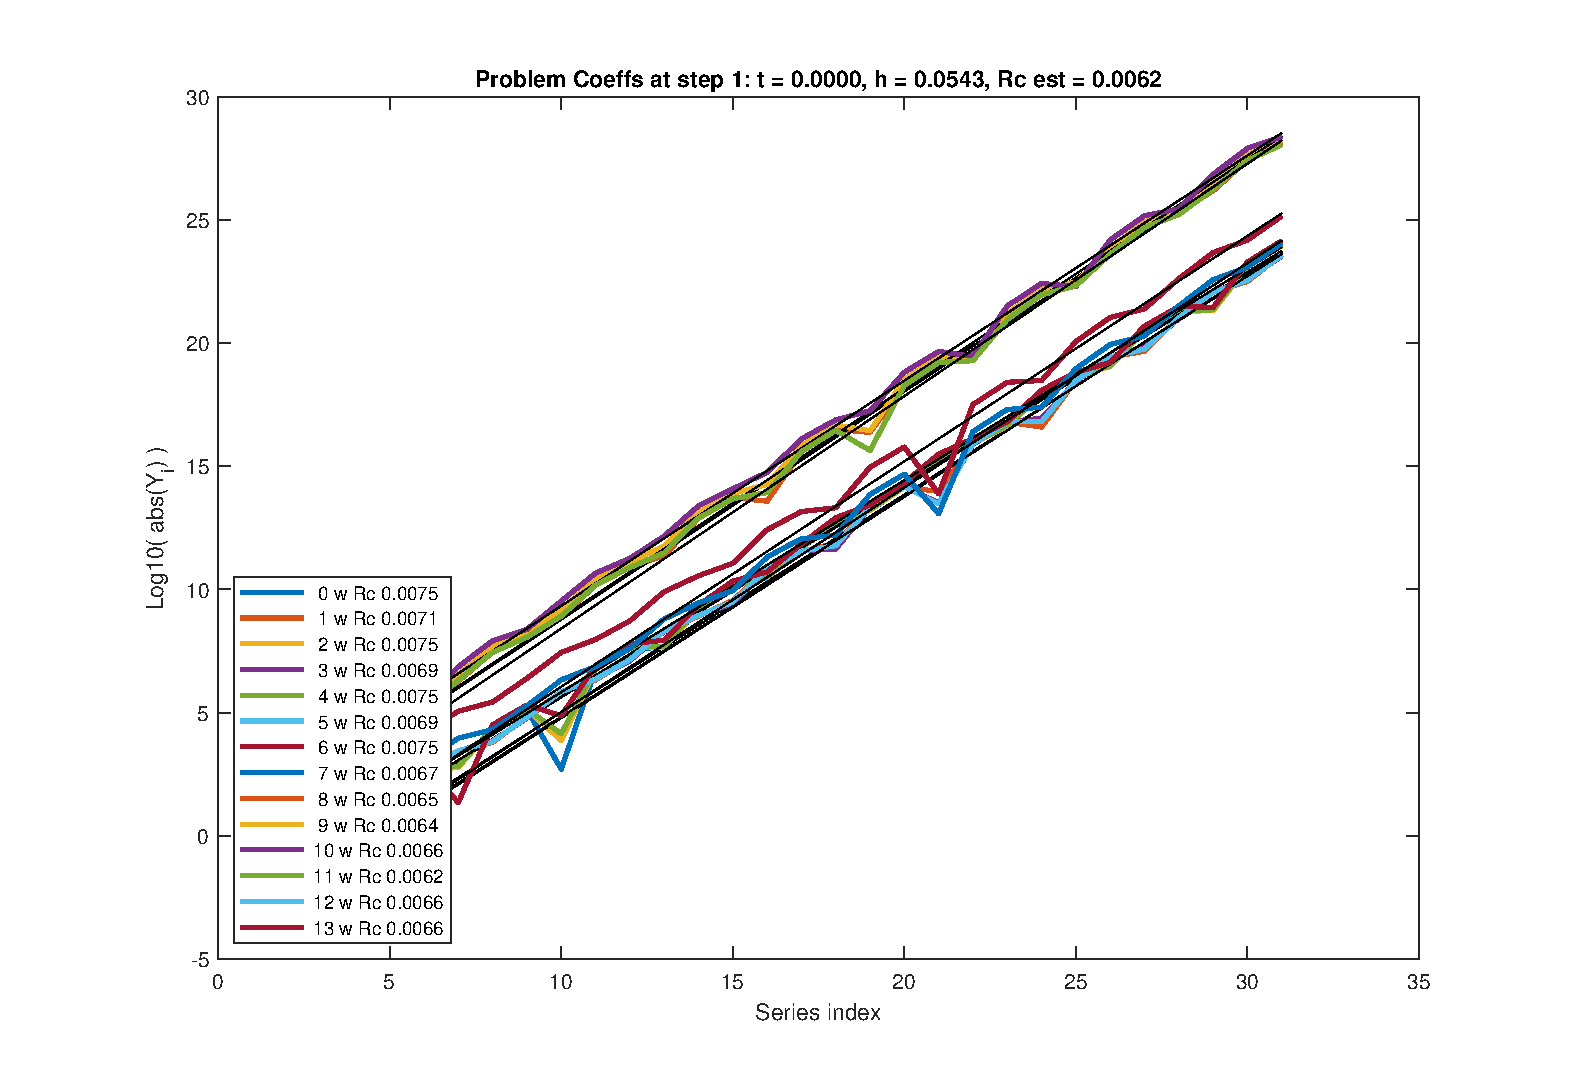
\includegraphics[width=.9\linewidth]{divergent.eps} %
  \caption{Top-line analysis shows divergent TS and rejected step}
\end{figure}

\end{frame}

\begin{frame}

\begin{figure}
  \centering
  \vspace{-0.4cm}
  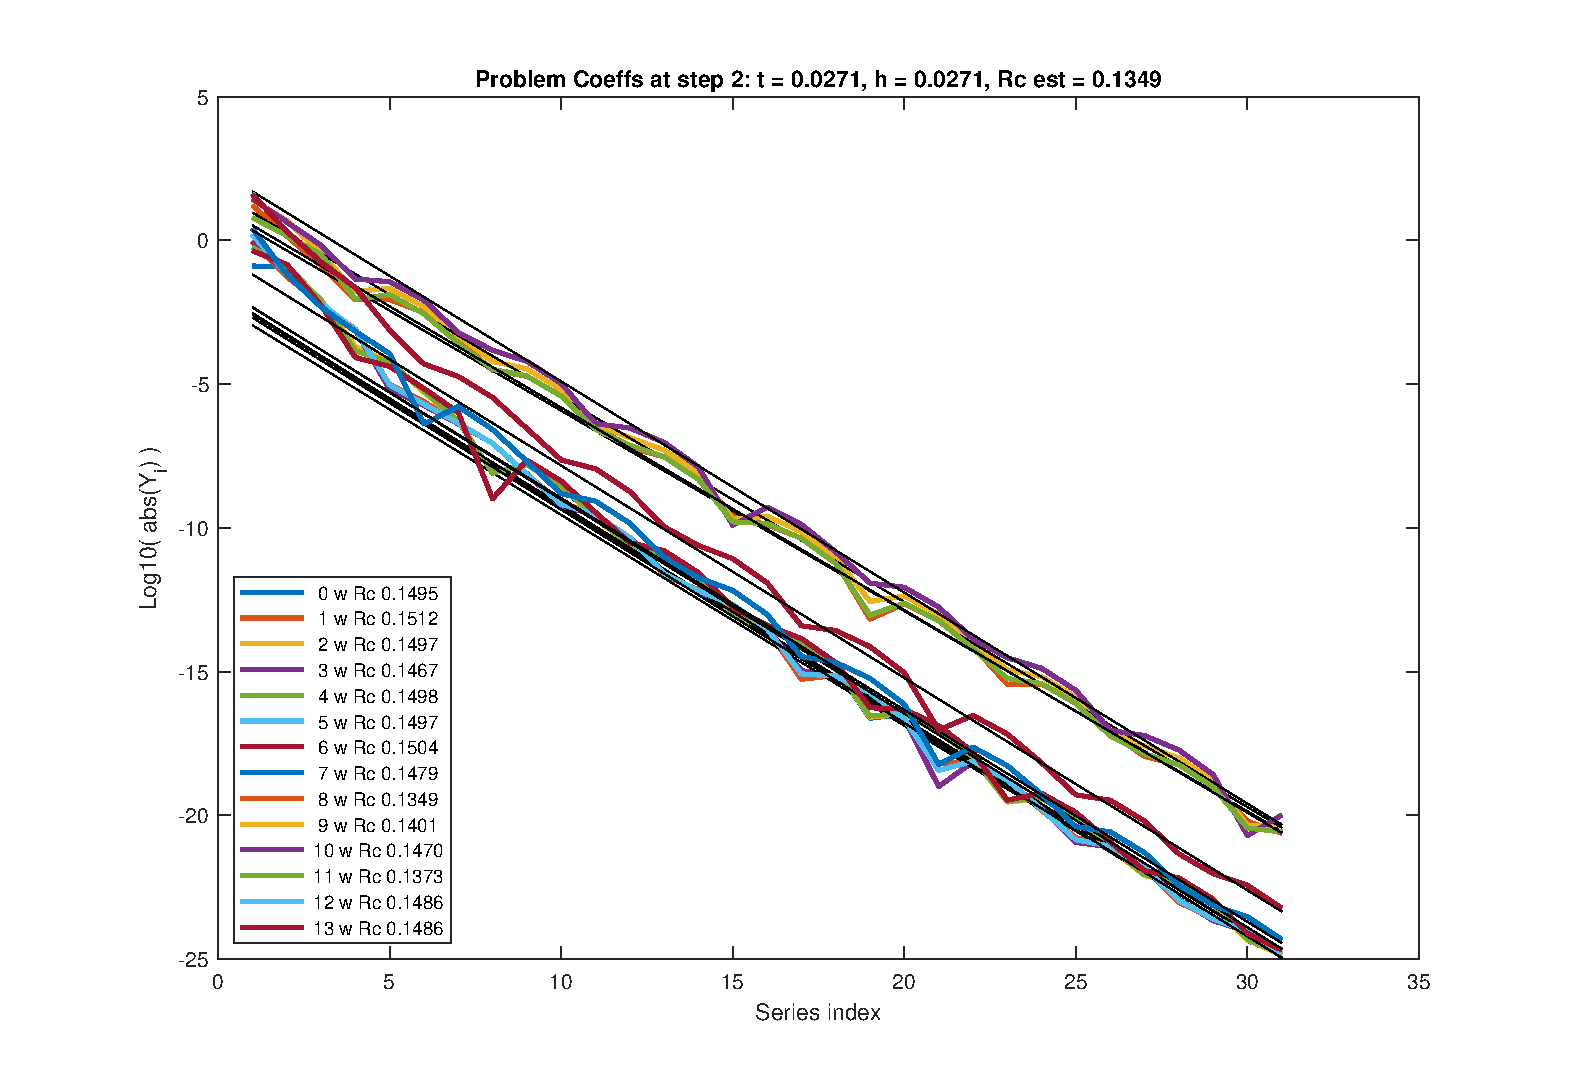
\includegraphics[width=.9\linewidth]{convergent.eps} %
  \caption{Top-line analysis indicates convergent TS and stepsize}
\end{figure}

\end{frame}

\begin{frame}{The ROC and its applications}

\begin{itemize}
  \item Chang and Corliss defined ROC top-line analysis method\\
    \EC{\footnotesize Chang and Corliss (1982)}

  \vspace{5mm}

  \item Taylor series methods\\
    \vspace{1mm}
    \EC{\footnotesize
      Jorba and Zou (2005)\\
      \vspace{1mm}
      Bergsma and Mooij (2016)\\
      \vspace{1mm}
      Chang and Corliss (1971)
    }
\end{itemize}

\end{frame}

\begin{frame}{Model refinement}{Assumptions, Theoretical Models, Instance Models, General Definitions, Data Definitions}

\begin{itemize}
  \item[A] real valued, sufficiently differentiable function in one real variable
  \item[A] Realize TCs or TS
  \item[] Fitting TS as data
  \item[] Assigning meaning to the fitting parameters, $\beta_1 + \text{idx} \beta_2$
  \item[] Convergence $\beta_2 < 0$ or divergence $\beta_2 > 0$
  \item[IM] ODE IVP solving
  \item[] The ROC $r_c = \text{abs}(t_{n+1} - t_{n}) / 10^{\beta_2}$
  \item[] The ROC as a stepsize
  \item[] This problem may be a candidate for Drasil after all
\end{itemize}


\end{frame}


\end{document}
